%-------------------------------------------------------%
\section{初期値・境界値データの作成:init} \label{sec:tutrial_real_init}
%-------------------------------------------------------%

\verb|init|ディレクトリに移動し、\scalerm によるシミュレーションに必要な初期値・境界値データを作成する。
\begin{verbatim}
 $ cd ${Tutorial_DIR}/real/experiment/init
 $ ls
    Makefile
    init.d01.conf
    init.launch.conf
    param.bucket.conf
    scale-rm_init
\end{verbatim}
ディレクトリの中には、\verb|init.d01.conf|という名前の設定ファイルが準備されている。\\
他に\verb|init.launch.conf|というファイルも存在するが、ここでは使用しない。
\verb|init.d01.conf|ファイルには、表\ref{tab:grids}に示すチュートリアル用の設定が
すでになされているが、\verb|pp.d01.conf|と同様に実験設定に応じて変更されたい。
初期値・境界値データの作成には、前節で作成した地形データを利用する。
これは、\verb|init.d01.conf|の中で、下記のように相対パスを用いて参照するように設定される。\\

\noindent {\gt
\ovalbox{
\begin{tabularx}{150mm}{l}
\verb|&PARAM_TOPO| \\
\verb|   TOPO_IN_BASENAME = "../pp/topo_d01",| \\
\verb|/| \\
 \\
\verb|&PARAM_LANDUSE| \\
\verb|   LANDUSE_IN_BASENAME = "../pp/landuse_d01",| \\
\verb|/| \\
\end{tabularx}
}}\\

\noindent その他に\verb|init.d01.conf|の設定の中で特に確認してほしいのは、
\namelist{PARAM_MKINIT_REAL_ATMOS}、
\namelist{PARAM_MKINIT_REAL_OCEAN}、
\namelist{PARAM_MKINIT_REAL_LAND}の内容である。\\

\noindent {\gt
\ovalbox{
\begin{tabularx}{150mm}{lX}
\verb|&PARAM_MKINIT_REAL_ATMOS| & \\
\verb| NUMBER_OF_FILES      = 2,|                                   & {\small ← 読み込むファイルの数} \\
\verb| FILETYPE_ORG         = "GrADS",|                             & {\small ← 表\ref{tab:inputdata_format}から選択する} \\
\verb| BASENAME_ORG         = "namelist.grads_boundary.FNL.grib1",| & \\
\verb| BASENAME_BOUNDARY    = "boundary_d01",|                      & {\small ← 境界値データの出力名} \\
\verb| BOUNDARY_UPDATE_DT   = 21600.0,|                             & {\small ← 入力データの時間間隔} \\
\verb| PARENT_MP_TYPE       = 3,|                                   & \\
\verb| USE_FILE_DENSITY     = .false.,|                             & {\small ← 親モデルの大気密度データを使うか} \\
\verb|/| \\
\\
\verb|&PARAM_MKINIT_REAL_OCEAN| & \\
\verb|   ..... 略 .....              |  & \\
\verb| INTRP_OCEAN_SFC_TEMP = "mask",|                              & {\small ← SSTの欠測値処理方法} \\
\verb| INTRP_OCEAN_TEMP     = "mask",|                              & {\small ← SSTの欠測値処理方法} \\
\verb|/| \\
\\
\verb|&PARAM_MKINIT_REAL_LAND| & \\
\verb|   ..... 略 .....              | & \\
\verb| USE_FILE_LANDWATER   = .true.,|                              & {\small ← 親モデルの土壌水分データを使うか} \\
\verb| INTRP_LAND_TEMP      = "mask",|                              & {\small ← 土壌温度の欠測値処理方法} \\
\verb| INTRP_LAND_WATER     = "fill",|                              & {\small ← 土壌水分の欠測値処理方法} \\
\verb| INTRP_LAND_SFC_TEMP  = "fill",|                              & {\small ← 地表面温度の欠測値処理方法} \\
\verb|/| \\
\end{tabularx}
}}\\

\noindent 気象場データのファイル形式は、\nmitem{FILETYPE_ORG}で指定する。
ここでは、{\grads}形式のデータを読み込むために``\verb|grads|''と与えている。
入力ファイルの詳細は、第\ref{sec:adv_datainput}節を参照されたい。

第\ref{sec:tutrial_real_data}節では、バイナリ形式に変換した入力データ(FNL)を準備したが、
今の作業ディレクトリにこのファイルへのリンクを張る。リンクを適切に張るためのスクリプトとして、
\verb|${Tutorial_DIR}/real/data|の中に\verb|"gradsinput-link_FNL.sh"|を用意している。
\begin{verbatim}
  $ cp ../../data/gradsinput-link_FNL.sh ./
  $ sh gradsinput-link_FNL.sh
\end{verbatim}
上記のコマンドを実行し、下記のリンクが作成されていれば成功である。\\

\noindent {\gt
\fbox{
\begin{tabularx}{150mm}{l}
\verb|ATM_00000.grd -> ../tools/FNL_output/200707/FNL_ATM_2007071418.grd| \\
\verb|ATM_00001.grd -> ../tools/FNL_output/200707/FNL_ATM_2007071500.grd| \\
\verb|LND_00000.grd -> ../tools/FNL_output/200707/FNL_LND_2007071418.grd| \\
\verb|LND_00001.grd -> ../tools/FNL_output/200707/FNL_LND_2007071500.grd| \\
\verb|SFC_00000.grd -> ../tools/FNL_output/200707/FNL_SFC_2007071418.grd| \\
\verb|SFC_00001.grd -> ../tools/FNL_output/200707/FNL_SFC_2007071500.grd| \\
\end{tabularx}
}}\\


次に、{\grads}形式のバイナリデータをSCALEで読み込むためのnamelistファイルを
\verb|init|ディレクトリへリンクする。
\begin{verbatim}
  $ ln -s ../../data/namelist.grads_boundary.FNL.2005053112-2016051106 ./
\end{verbatim}
%
上記の準備が終わったら、4つのMPIプロセスを使用して\verb|scale-rm_init|を実行する。
\begin{verbatim}
 $ mpirun -n 4 ./scale-rm_init init.d01.conf
\end{verbatim}

正常にジョブが終了すれば、以下のファイルが生成される。
\begin{verbatim}
 $ ls
    boundary_d01.pe000000.nc
    boundary_d01.pe000001.nc
    boundary_d01.pe000002.nc
    boundary_d01.pe000003.nc
    init_d01_20070714-180000.000.pe000000.nc
    init_d01_20070714-180000.000.pe000001.nc
    init_d01_20070714-180000.000.pe000002.nc
    init_d01_20070714-180000.000.pe000003.nc
    init_LOG_d01.pe000000
\end{verbatim}
\verb|init_LOG_d01.pe000000|はログファイルであり、
処理が正常に完了していれば、ファイルの最後に\\

\noindent {\small {\gt
\fbox{
\begin{tabularx}{150mm}{l}
 +++++ finalize MPI...\\
 +++++ MPI is peacefully finalized\\
\end{tabularx}
}}}\\

\noindent
という内容が出力される。
\verb|boundary_d01.pe######.nc|は境界値データ、
\verb|init_d01_20070714-180000.000.pe######.nc|は初期値データであり、
それぞれのファイルサイズは約18.9 MB、約12.6 MB である。、
ここで、\verb|######|はMPIプロセス番号を表す。

%% サポート外
\vspace{1cm}
\noindent {\Large\em OPTION} \hrulefill \\
「gpview」がインストールされている場合には,以下のコマンドによって、
初期値と境界値が正しく作成されているかを確認できる。

\begin{verbatim}
 $ gpvect --scalar --slice z=1500 --nocont --aspect=1 --range=0.002:0.016 --int 0.001     \
          --xintv=10 --yintv=10 --unit_vect init_d01_20070714-180000.000.pe00*@QV         \
          init_d01_20070714-180000.000.pe00*@MOMX init_d01_20070714-180000.000.pe00*@MOMY \
          --title "QV, MOMX, MOMY"
\end{verbatim}
処理が正常に終了していれば、図\ref{fig:init}と同様の図が得られる。

\begin{figure}[h]
\begin{center}
  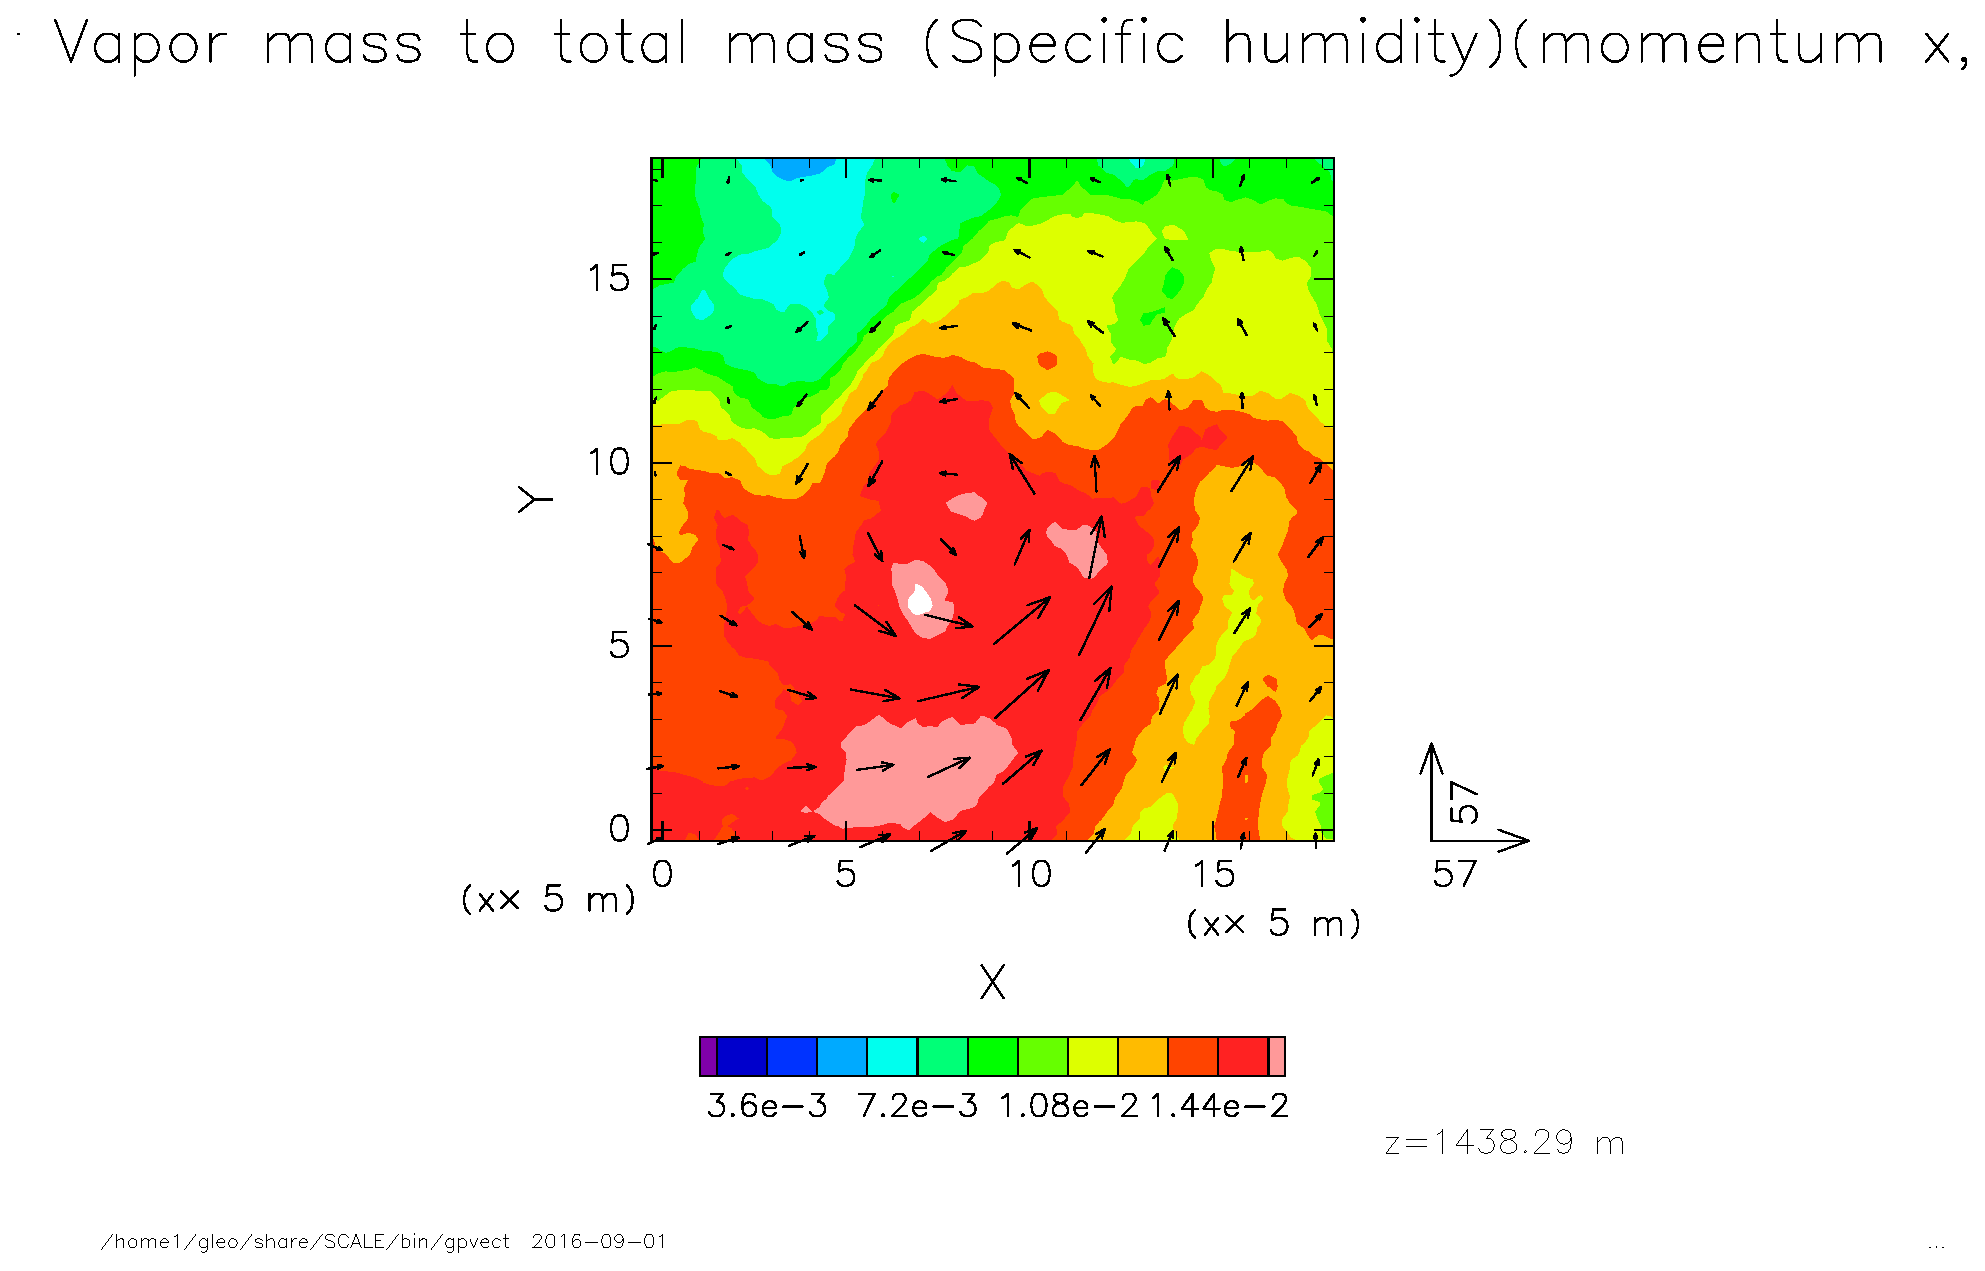
\includegraphics[width=0.9\hsize]{./figure/real_init_qv-momxy.eps}\\
  \caption{チュートリアル実験における初期場の様子($z=$1500 m)。
           色は比湿、ベクトルは水平運動量フラックスを表す。}
  \label{fig:init}
\end{center}
\end{figure}

